%%Line 1810 uncomment

\documentclass[2dCFT-lecture.tex]{subfiles}
%\usepackage{subfiles}
%\usepackage{epsfig}
%\usepackage{amsmath}
%\usepackage{amssymb}
%\usepackage{amsthm}
%\usepackage{indentfirst}
%\usepackage{xspace}
%\usepackage{multirow}
%\usepackage{hyperref}
%\usepackage{xcolor}
%\usepackage{verbatim}
%%\hypersetup{colorlinks=true,urlcolor=darkred,linkcolor=darkred,citecolor=darkred}
%%\usepackage{verbatim}
%\usepackage[letterpaper,margin=0.9in,headheight=15pt]{geometry}
%\usepackage{mathpazo}
%\usepackage{authblk}
%\usepackage{empheq}
%\usepackage{feynmp}
%\usepackage{graphicx}
%\usepackage[matrix,arrow]{xy}
%\usepackage{young}
%\usepackage[vcentermath]{youngtab}
%\usepackage{slashed}
%%\usepackage{fontds}
%%
%\usepackage{bbm}
%\usepackage{youngtab}
%\usepackage{rotfloat}
%\usepackage{stmaryrd}
%\usepackage{amsfonts,amssymb,amsmath}
%\usepackage{tikz-cd}
%\usepackage{thmtools}
%\usepackage{dashrule}
%\usepackage[missing=]{gitinfo2}
%\usepackage{fancyhdr}
%\usepackage{mdframed}
%
%\usepackage{subfiles}



%
%
%\definecolor{darkblue}{rgb}{0.1,0.1,0.7}
%\definecolor{darkred}{rgb}{0.5,0.1,0.1}
%\definecolor{darkgreen}{rgb}{0.0,0.42,0.06}
%\hypersetup{colorlinks=true,urlcolor=darkred,linkcolor=darkblue,citecolor=darkred}
%\definecolor{shadecolor}{rgb}{0.85,0.85,0.85}
%
%
%
%% theorem environments
%\declaretheoremstyle[spaceabove=0.25cm,spacebelow=0.25cm,notefont=\normalfont\bfseries, notebraces={(}{)}]{theorem}
%\declaretheoremstyle[spaceabove=0.25cm,spacebelow=0.25cm,bodyfont=\normalfont,notefont=\normalfont\bfseries, notebraces={(}{)}]{noital}
%\declaretheoremstyle[spaceabove=0.25cm,spacebelow=0.25cm,bodyfont=\normalfont\color{darkgreen},notefont=\normalfont\bfseries, notebraces={(}{)}]{green}
%\declaretheoremstyle[spaceabove=0.25cm,spacebelow=0.25cm,bodyfont=\normalfont,notefont=\normalfont\bfseries,qed=$\qedsymbol$,notebraces={(}{)}]{proofstyle}
%
%\declaretheorem[name=Theorem,numberwithin=section,style=theorem]{thm}
%\declaretheorem[name=Proposition,sibling=thm,style=theorem]{prop}
%\declaretheorem[name=Corollary,sibling=thm,style=theorem]{cor}
%\declaretheorem[name=Lemma,sibling=thm,style=theorem]{lem}
%\declaretheorem[name=Remark,style=theorem,numbered=no]{rem}
%\declaretheorem[name=Definition,sibling=thm,style=noital]{defn}
%\declaretheorem[name=Example,sibling=thm,style=noital]{example}
%\declaretheorem[name=Exercise,numberwithin=section,style=green]{exercise}
%\declaretheorem[name=Proof,style=proofstyle,numbered=no]{pf}
%
%\numberwithin{equation}{section}
%
%
%\usepackage[most,listings]{tcolorbox}
%\tcbuselibrary{breakable}
%
%\tcbset{colframe=white}
%
%\def \bthm {\begin{tcolorbox}[breakable,boxsep=5pt,left=0pt,right=0pt,top=0pt,bottom=0pt]\begin{thm}}
%\def \ethm {\end{thm}\end{tcolorbox}}
%\def \bprop {\begin{tcolorbox}[breakable,boxsep=5pt,left=0pt,right=0pt,top=0pt,bottom=0pt]\begin{prop}}
%\def \eprop {\end{prop}\end{tcolorbox}}
%\def \blem {\begin{tcolorbox}[breakable,boxsep=5pt,left=0pt,right=0pt,top=0pt,bottom=0pt]\begin{lem}}
%\def \elem {\end{lem}\end{tcolorbox}}
%\def \bcor {\begin{tcolorbox}[breakable,boxsep=5pt,left=0pt,right=0pt,top=0pt,bottom=0pt]\begin{cor}}
%\def \ecor {\end{cor}\end{tcolorbox}}
%\def \bdefn {\begin{tcolorbox}[breakable,boxsep=5pt,left=0pt,right=0pt,top=0pt,bottom=0pt]\begin{defn}}
%\def \edefn {\end{defn}\end{tcolorbox}}
%\def \bexample {\begin{tcolorbox}[colback=blue!2,breakable,boxsep=5pt,left=0pt,right=0pt,top=0pt,bottom=0pt]\begin{example}}
%\def \eexample {\end{example}\end{tcolorbox}}
%\def \brem {\begin{tcolorbox}[colback=blue!2,breakable,boxsep=5pt,left=0pt,right=0pt,top=0pt,bottom=0pt]\begin{rem}}
%\def \erem {\end{rem}\end{tcolorbox}}
%
%
%%%%%%%%  Greek letters %%%%%%%%%%%%%%%%%%
%\def\a{\alpha}
%\def\b{\beta}
%\def\c{\gamma} \def\g{\gamma}
%\def\d{\delta}
%\def\e{\epsilon}          
%\def\f{\phi}              
%\def\vf{\varphi}  \def\tvf{\tilde{\varphi}}
%\def\vp{\varphi}
%\def\h{\eta}
%\def\i{\iota}
%\def\j{\psi}
%\def\k{\kappa}    
%\def\m{\mu}
%\def\n{\nu}
%\def\o{\omega}  \def\w{\omega}
%\def\q{\theta}  \def\th{\theta}                  
%\def\r{\rho}                                     
%\def\s{\sigma}                                  
%\def\t{\tau}
%\def\u{\upsilon}
%\def\x{\xi}
%\def\z{\zeta} 
%
%\def\A{\Alpha}
%\def\B{\Beta}
%\def\G{\Gamma}
%\def\D{\Delta}
%\def\E{\Epsilon}         
%\def\F{Phi}          
%\def\h{\eta}
%\def\I{\Iota}
%\def\J{Psi}
%%\def\K{\Kappa}                    
%\def\L{\Lambda}
%\def\M{\Mu}
%\def\N{\Nu}
%\def\O{\Omega}  \def\w{\omega}
%\def\Q{\Theta}  \def\Th{\Theta}                  
%\def\R{\Rho}                                    
%\def\Si{\Sigma}                                   
%\def\T{\Tau}
%\def\Up{\Upsilon}
%\def\X{\Xi}
%\def\Z{\Zeta}
%
%
%
%
%%%%%%%%%%%%% math fonts %%%%%%%%%%%%%%%%%%%%%%%%%%%%%%%%%%%%%
%%
%%---------- mathbb font --------------------------------
%%
%
%\newcommand{\bA}{\ensuremath{\mathbb{A}}}
%\newcommand{\bB}{\ensuremath{\mathbb{B}}}
%\newcommand{\bC}{\ensuremath{\mathbb{C}}}
%\newcommand{\bD}{\ensuremath{\mathbb{D}}}
%\newcommand{\bE}{\ensuremath{\mathbb{E}}}
%\newcommand{\bF}{\ensuremath{\mathbb{F}}}
%\newcommand{\bG}{\ensuremath{\mathbb{G}}}
%\newcommand{\bH}{\ensuremath{\mathbb{H}}}
%\newcommand{\bI}{\ensuremath{\mathbb{I}}}
%\newcommand{\bJ}{\ensuremath{\mathbb{J}}}
%\newcommand{\bK}{\ensuremath{\mathbb{K}}}
%\newcommand{\bL}{\ensuremath{\mathbb{L}}}
%\newcommand{\bM}{\ensuremath{\mathbb{M}}}
%\newcommand{\bN}{\ensuremath{\mathbb{N}}}
%\newcommand{\bO}{\ensuremath{\mathbb{O}}}
%\newcommand{\bP}{\ensuremath{\mathbb{P}}}
%\newcommand{\bQ}{\ensuremath{\mathbb{Q}}}
%\newcommand{\bR}{\ensuremath{\mathbb{R}}}
%\newcommand{\bS}{\ensuremath{\mathbb{S}}}
%\newcommand{\bT}{\ensuremath{\mathbb{T}}}
%\newcommand{\bU}{\ensuremath{\mathbb{U}}}
%\newcommand{\bV}{\ensuremath{\mathbb{V}}}
%\newcommand{\bW}{\ensuremath{\mathbb{W}}}
%\newcommand{\bX}{\ensuremath{\mathbb{X}}}
%\newcommand{\bY}{\ensuremath{\mathbb{Y}}}
%\newcommand{\bZ}{\ensuremath{\mathbb{Z}}}
%
%
%
%%
%%---------- mathbf font --------------------------------
%%
%
%
%\newcommand{\bfA}{\ensuremath{\mathbf{A}}}
%\newcommand{\bfB}{\ensuremath{\mathbf{B}}}
%\newcommand{\bfC}{\ensuremath{\mathbf{C}}}
%\newcommand{\bfD}{\ensuremath{\mathbf{D}}}
%\newcommand{\bfE}{\ensuremath{\mathbf{E}}}
%\newcommand{\bfF}{\ensuremath{\mathbf{F}}}
%\newcommand{\bfG}{\ensuremath{\mathbf{G}}}
%\newcommand{\bfH}{\ensuremath{\mathbf{H}}}
%\newcommand{\bfI}{\ensuremath{\mathbf{I}}}
%\newcommand{\bfJ}{\ensuremath{\mathbf{J}}}
%\newcommand{\bfK}{\ensuremath{\mathbf{K}}}
%\newcommand{\bfL}{\ensuremath{\mathbf{L}}}
%\newcommand{\bfM}{\ensuremath{\mathbf{M}}}
%\newcommand{\bfN}{\ensuremath{\mathbf{N}}}
%\newcommand{\bfO}{\ensuremath{\mathbf{O}}}
%\newcommand{\bfP}{\ensuremath{\mathbf{P}}}
%\newcommand{\bfQ}{\ensuremath{\mathbf{Q}}}
%\newcommand{\bfR}{\ensuremath{\mathbf{R}}}
%\newcommand{\bfS}{\ensuremath{\mathbf{S}}}
%\newcommand{\bfT}{\ensuremath{\mathbf{T}}}
%\newcommand{\bfU}{\ensuremath{\mathbf{U}}}
%\newcommand{\bfV}{\ensuremath{\mathbf{V}}}
%\newcommand{\bfW}{\ensuremath{\mathbf{W}}}
%\newcommand{\bfX}{\ensuremath{\mathbf{X}}}
%\newcommand{\bfY}{\ensuremath{\mathbf{Y}}}
%\newcommand{\bfZ}{\ensuremath{\mathbf{Z}}}
%
%
%
%
%%
%%---------- mathcal font -----------------------------
%%
%
%\newcommand{\scA}{\ensuremath{\mathscr{A}}}
%\newcommand{\scB}{\ensuremath{\mathscr{B}}}
%\newcommand{\scC}{\ensuremath{\mathscr{C}}}
%\newcommand{\scD}{\ensuremath{\mathscr{D}}}
%\newcommand{\scE}{\ensuremath{\mathscr{E}}}
%\newcommand{\scF}{\ensuremath{\mathscr{F}}}
%\newcommand{\scG}{\ensuremath{\mathscr{G}}}
%\newcommand{\scH}{\ensuremath{\mathscr{H}}}
%\newcommand{\scI}{\ensuremath{\mathscr{I}}}
%\newcommand{\scJ}{\ensuremath{\mathscr{J}}}
%\newcommand{\scK}{\ensuremath{\mathscr{K}}}
%\newcommand{\scL}{\ensuremath{\mathscr{L}}}
%\newcommand{\scM}{\ensuremath{\mathscr{M}}}
%\newcommand{\scN}{\ensuremath{\mathscr{N}}}
%\newcommand{\scO}{\ensuremath{\mathscr{O}}}
%\newcommand{\scP}{\ensuremath{\mathscr{P}}}
%\newcommand{\scQ}{\ensuremath{\mathscr{Q}}}
%\newcommand{\scR}{\ensuremath{\mathscr{R}}}
%\newcommand{\scS}{\ensuremath{\mathscr{S}}}
%\newcommand{\scT}{\ensuremath{\mathscr{T}}}
%\newcommand{\scU}{\ensuremath{\mathscr{U}}}
%\newcommand{\scV}{\ensuremath{\mathscr{V}}}
%\newcommand{\scW}{\ensuremath{\mathscr{W}}}
%\newcommand{\scX}{\ensuremath{\mathscr{X}}}
%\newcommand{\scY}{\ensuremath{\mathscr{Y}}}
%\newcommand{\scZ}{\ensuremath{\mathscr{Z}}}
%
%%
%%---------- mathfrak font -----------------------------
%%
%
%\newcommand{\frakA}{\ensuremath{\mathfrak{A}}}
%\newcommand{\frakB}{\ensuremath{\mathfrak{B}}}
%\newcommand{\frakC}{\ensuremath{\mathfrak{C}}}
%\newcommand{\frakD}{\ensuremath{\mathfrak{D}}}
%\newcommand{\frakE}{\ensuremath{\mathfrak{E}}}
%\newcommand{\frakF}{\ensuremath{\mathfrak{F}}}
%\newcommand{\frakG}{\ensuremath{\mathfrak{G}}}
%\newcommand{\frakH}{\ensuremath{\mathfrak{H}}}
%\newcommand{\frakI}{\ensuremath{\mathfrak{I}}}
%\newcommand{\frakJ}{\ensuremath{\mathfrak{J}}}
%\newcommand{\frakK}{\ensuremath{\mathfrak{K}}}
%\newcommand{\frakL}{\ensuremath{\mathfrak{L}}}
%\newcommand{\frakM}{\ensuremath{\mathfrak{M}}}
%\newcommand{\frakN}{\ensuremath{\mathfrak{N}}}
%\newcommand{\frakO}{\ensuremath{\mathfrak{O}}}
%\newcommand{\frakP}{\ensuremath{\mathfrak{P}}}
%\newcommand{\frakQ}{\ensuremath{\mathfrak{Q}}}
%\newcommand{\frakR}{\ensuremath{\mathfrak{R}}}
%\newcommand{\frakS}{\ensuremath{\mathfrak{S}}}
%\newcommand{\frakT}{\ensuremath{\mathfrak{T}}}
%\newcommand{\frakU}{\ensuremath{\mathfrak{U}}}
%\newcommand{\frakV}{\ensuremath{\mathfrak{V}}}
%\newcommand{\frakW}{\ensuremath{\mathfrak{W}}}
%\newcommand{\frakX}{\ensuremath{\mathfrak{X}}}
%\newcommand{\frakY}{\ensuremath{\mathfrak{Y}}}
%\newcommand{\frakZ}{\ensuremath{\mathfrak{Z}}}
%\newcommand{\fraka}{\ensuremath{\mathfrak{a}}}
%\newcommand{\frakb}{\ensuremath{\mathfrak{b}}}
%\newcommand{\frakc}{\ensuremath{\mathfrak{c}}}
%\newcommand{\frakd}{\ensuremath{\mathfrak{d}}}
%\newcommand{\frake}{\ensuremath{\mathfrak{e}}}
%\newcommand{\frakf}{\ensuremath{\mathfrak{f}}}
%\newcommand{\frakg}{\ensuremath{\mathfrak{g}}}
%\newcommand{\frakh}{\ensuremath{\mathfrak{h}}}
%\newcommand{\fraki}{\ensuremath{\mathfrak{i}}}
%\newcommand{\frakj}{\ensuremath{\mathfrak{j}}}
%\newcommand{\frakk}{\ensuremath{\mathfrak{k}}}
%\newcommand{\frakl}{\ensuremath{\mathfrak{l}}}
%\newcommand{\frakm}{\ensuremath{\mathfrak{m}}}
%\newcommand{\frakn}{\ensuremath{\mathfrak{n}}}
%\newcommand{\frako}{\ensuremath{\mathfrak{o}}}
%\newcommand{\frakp}{\ensuremath{\mathfrak{p}}}
%\newcommand{\frakq}{\ensuremath{\mathfrak{q}}}
%\newcommand{\frakr}{\ensuremath{\mathfrak{r}}}
%\newcommand{\fraks}{\ensuremath{\mathfrak{s}}}
%\newcommand{\frakt}{\ensuremath{\mathfrak{t}}}
%\newcommand{\fraku}{\ensuremath{\mathfrak{u}}}
%\newcommand{\frakv}{\ensuremath{\mathfrak{v}}}
%\newcommand{\frakw}{\ensuremath{\mathfrak{w}}}
%\newcommand{\frakx}{\ensuremath{\mathfrak{x}}}
%\newcommand{\fraky}{\ensuremath{\mathfrak{y}}}
%\newcommand{\frakz}{\ensuremath{\mathfrak{z}}}
%\newcommand{\fraksl}{\ensuremath{\mathfrak{sl}}}
%\newcommand{\frakso}{\ensuremath{\mathfrak{so}}}
%\newcommand{\fraksp}{\ensuremath{\mathfrak{sp}}}
%
%%%%%%%%%%%%%  Calligraphic, Roman and Maths integers %%%%%%%%%%%%%%%%%%
%
%\newcommand{\cA}{\mathcal{A}}
%\newcommand{\cB}{\mathcal{B}}
%\newcommand{\cC}{\mathcal{C}}
%\newcommand{\cD}{\mathcal{D}}
%\newcommand{\cE}{\mathcal{E}}
%\newcommand{\cF}{\mathcal{F}}
%\newcommand{\cG}{\mathcal{G}}
%\newcommand{\cH}{\mathcal{H}}
%\newcommand{\cJ}{\mathcal{J}}
%\newcommand{\cK}{\mathcal{K}}
%\newcommand{\cL}{\mathcal{L}}
%\newcommand{\cM}{\mathcal{M}}
%\newcommand{\cN}{\mathcal{N}}
%\newcommand{\cO}{\mathcal{O}}
%\newcommand{\cP}{\mathcal{P}}
%\newcommand{\cQ}{\mathcal{Q}}
%\newcommand{\cS}{\mathcal{S}}
%\newcommand{\cU}{\mathcal{U}}
%\newcommand{\cX}{\mathcal{X}}
%\newcommand{\cY}{\mathcal{Y}}
%\newcommand{\cW}{\mathcal{W}}
%\newcommand{\cR}{\mathcal{R}}
%\newcommand{\cT}{\mathcal{T}}
%\newcommand{\cZ}{\mathcal{Z}}
%
%
%%%%%%%%%%%%% mathsf%%%%%%%%%%%%%%%%%%
%
%
%\newcommand{\sfA}{\ensuremath{\mathsf{A}}}
%\newcommand{\sfB}{\ensuremath{\mathsf{B}}}
%\newcommand{\sfC}{\ensuremath{\mathsf{C}}}
%\newcommand{\sfD}{\ensuremath{\mathsf{D}}}
%\newcommand{\sfE}{\ensuremath{\mathsf{E}}}
%\newcommand{\sfF}{\ensuremath{\mathsf{F}}}
%\newcommand{\sfG}{\ensuremath{\mathsf{G}}}
%\newcommand{\sfH}{\ensuremath{\mathsf{H}}}
%\newcommand{\sfJ}{\ensuremath{\mathsf{J}}}
%\newcommand{\sfK}{\ensuremath{\mathsf{K}}}
%\newcommand{\sfL}{\ensuremath{\mathsf{L}}}
%\newcommand{\sfM}{\ensuremath{\mathsf{M}}}
%\newcommand{\sfN}{\ensuremath{\mathsf{N}}}
%\newcommand{\sfO}{\ensuremath{\mathsf{O}}}
%\newcommand{\sfP}{\ensuremath{\mathsf{P}}}
%\newcommand{\sfQ}{\ensuremath{\mathsf{Q}}}
%\newcommand{\sfS}{\ensuremath{\mathsf{S}}}
%\newcommand{\sfU}{\ensuremath{\mathsf{U}}}
%\newcommand{\sfX}{\ensuremath{\mathsf{X}}}
%\newcommand{\sfY}{\ensuremath{\mathsf{Y}}}
%\newcommand{\sfW}{\ensuremath{\mathsf{W}}}
%\newcommand{\sfR}{\ensuremath{\mathsf{R}}}
%\newcommand{\sfT}{\ensuremath{\mathsf{T}}}
%\newcommand{\sfZ}{\ensuremath{\mathsf{Z}}}
%
%%%%%%%%%%%%%  Special letters for Lie groups %%%%%%%%%%%%%%%%%%
%
%\newcommand{\biA}{{\mathbi{A}}}
%\newcommand{\biB}{{\mathbi{B}}}
%\newcommand{\biC}{{\mathbi{C}}}
%\newcommand{\biD}{{\mathbi{D}}}
%\newcommand{\biE}{{\mathbi{E}}}
%\newcommand{\biF}{{\mathbi{F}}}
%\newcommand{\biG}{{\mathbi{G}}}
%\newcommand{\biH}{{\mathbi{H}}}
%\newcommand{\biJ}{{\mathbi{J}}}
%\newcommand{\biK}{{\mathbi{K}}}
%\newcommand{\biL}{{\mathbi{L}}}
%\newcommand{\biM}{{\mathbi{M}}}
%\newcommand{\biN}{{\mathbi{N}}}
%\newcommand{\biO}{{\mathbi{O}}}
%\newcommand{\biP}{{\mathbi{P}}}
%\newcommand{\biQ}{{\mathbi{Q}}}
%\newcommand{\biS}{{\mathbi{S}}}
%\newcommand{\biU}{{\mathbi{U}}}
%\newcommand{\biX}{{\mathbi{X}}}
%\newcommand{\biY}{{\mathbi{Y}}}
%\newcommand{\biV}{{\mathbi{V}}}
%\newcommand{\biW}{{\mathbi{W}}}
%\newcommand{\biR}{{\mathbi{R}}}
%\newcommand{\biT}{{\mathbi{T}}}
%\newcommand{\biZ}{{\mathbi{Z}}}
%
%
%
%
%%%%%%%%%%%%%%%%%%%%%%%%%%%%%%%%%%%%%%%%%%%%%%%%%%%%%%%%%%%%%%%%%
%\newcommand{\SU}{\mathrm{SU}}
%\newcommand{\SO}{\mathrm{SO}}
%\newcommand{\SL}{\mathrm{SL}}
%\newcommand{\GL}{\mathrm{GL}}
%\newcommand{\Sp}{\mathrm{Sp}}
%\newcommand{\U}{\mathrm{U}}
%\newcommand{\ul}{\mathrm{u}}
%\newcommand{\Spin}{\mathrm{Spin}}
%\newcommand{\Pin}{\mathrm{Pin}}
%%%%%%%%%%%%%%%%%%%%%%%%%%%%%%%%%%%%%%%%%%%%%%%%%%%%%%%%%%%%%%%%%
%
%
%
%
%
%\renewcommand{\Im}{{\rm Im}}
%\renewcommand{\Re}{{\rm Re}}
%\newcommand{\Tr}{\mbox{Tr}}
%\newcommand{\Pf}{\mbox{Pf}}
%\newcommand{\sgn}{\mbox{sgn}}
%\newcommand{\Vir}{{\rm Vir}}
%\newcommand{\Li}{{\rm Li}}
%
%
%
%%\def\cD{{\cal D}}
%%\def\cA{{\cal A}}
%%\def\cN{{\cal N}}
%%\def\cS{{\cal S}}
%%\def\cD{{\cal D}}
%%\def\cA{{\cal A}}
%%%%%%%%%%%%%%%%%%%%%%%%%%%%%%%%%%%%%%%%%%%%%%%%%%%%%%%%%%%%%%%%%
%
%
%\newcommand{\valp}{{\vec\alpha}}
%\newcommand{\vbet}{{\vec\beta}}
%\newcommand{\vgam}{{\vec\gamma}}
%\newcommand{\vrho}{{\vec\rho}}
%\newcommand{\vome}{{\vec\omega}}
%\newcommand{\vlam}{{\vec\lambda}}
%\newcommand{\vphi}{{\vec\varphi}}
%\newcommand{\va}{{\vec a}}
%\newcommand{\vb}{{\vec b}}
%\newcommand{\ve}{{\vec e}}
%\newcommand{\vx}{{\vec x}}
%\newcommand{\vW}{{\vec W}}
%\newcommand{\vY}{{\vec Y}}
%\newcommand{\vha}{{\vec{\hat a}}}
%\newcommand{\vhb}{{\vec{\hat b}}}
%\newcommand{\vhc}{{\vec{\hat c}}}
%
%%%%%%%%%%%%%%%%%%%%%%%%%%%%%%%%%%%%%%%%%%%%%%%%%%%%%%%%%%%%%%%%%
%
%
%
%\newcommand{\dalpha}{{\dot \alpha}}
%\newcommand{\dbeta}{{\dot \beta}}
%\newcommand{\dgamma}{{\dot \gamma}}
%\newcommand{\dmu}{{\dot \mu}}
%\newcommand{\dnu}{{\dot \nu}}
%\newcommand{\drho}{{\dot \rho}}
%\newcommand{\dsigma}{{\dot \sigma}}
%\newcommand{\dlambda}{{\dot \lambda}}
%\newcommand{\dtau}{{\dot \tau}}
%\newcommand{\ha}{{\hat a}}
%\newcommand{\hb}{{\hat b}}
%\newcommand{\hc}{{\hat c}}
%\newcommand{\hj}{j^\circ}
%\newcommand{\vh}{{\vec h}}
%\newcommand{\vm}{{\vec m}}
%\newcommand{\vn}{{\vec n}}
%\newcommand{\vl}{{\vec l}}
%
%\newcommand{\HK}{{hyper-K\"ahler }}
%\newcommand{\K}{{K\"ahler }}
%\newcommand{\pl}{\textrm{pl}}
%\newcommand{\Ind}{\textrm{Ind}}
%
%
%
%
%\def \be  {\begin{equation}}
%\def \ee  {\end{equation}}
%\def \bea {\begin{equation}\begin{aligned}}
%\def \eea {\end{aligned}\end{equation}}
%\def \ba  {\begin{eqnarray}}
%\def \ea  {\end{eqnarray}}
%
%
%
% 


\def\wt{\widetilde}
%\def\bZ{{\bar{z}}}






%
%
%
%\usepackage{accents}
%\newcommand*{\dt}[1]{%
%  \accentset{\mbox{\large\bfseries .}}{#1}}
%\newcommand*{\ddt}[1]{%
%  \accentset{\mbox{\large\bfseries .\hspace{-0.25ex}.}}{#1}}
%
%\newcommand{\Spec}{\operatorname{Spec}\nolimits}
%\newcommand{\Gr}{\mathrm{Gr}}
%
%\newcommand{\Hom}{\textrm{Hom}}
%\newcommand{\End}{\textrm{End}}
%\def\BunG{{\text{Bun}_G}}
%%\def\bfN{{\text{Nilp}}}
%\def\Bcc{{\mathfrak{B}_{cc}}}
%
%
%
%
%\def\MF{{\cM_\text{flat}}}
%\def\MH{{{\cM}_H}}
%\def\SH{\mathbi{S}\!\ddt{\mathbi{H}}}
%\def\HH{\ddt{\mathbi{H}}}
%\def\WW{ \ddt{\mathbi{W}}}
%\def\BB{\ddt{\mathbi{B}}\mathbi{r}}
%\def\wh{\widehat}
%\def\id{\mathrm{id}}
%\def\Td{\mathrm{Td}}
%
%
%
%\newcommand{\MyRed}{\color [rgb]{0.9,0,0}}
%\newcommand{\MyGreen}{\color [rgb]{0,0.5,0}}
%\newcommand{\MyBlue}{\color [rgb]{0,0,0.8}}
%\newcommand{\MyBrown}{\color [rgb]{0.8,0.3,0.2}}
%\newcommand{\MyPurple}{\color [rgb]{0.6,0.0,0.7}}
%
%
%\def\SN#1{{\MyRed [SN: #1]}}
%


%\title{Introduction to 2d conformal field theories}
%\date{}
%\author{Satoshi Nawata\cr email \href{mailto:snawata@gmail.com}{snawata@gmail.com} }
%%\author[2]{Anindya Dey}
%%\author[3]{Gregory W. Moore}
%\affil{Department of Physics and Center for Field Theory and Particle Physics, Fudan University, 220
%Handan Road, 200433 Shanghai, China}




\begin{document}
%\maketitle
%\abstract{These are lecture notes on 2d conformal field theories in Fall 2018. If you find typos, please email me. }
%


\setcounter{tocdepth}{2}
%\maketitle
\section{Introduction}




Conformal field theories have been at the centre of much attention
during the last few decades since they are relevant for at least
three different areas of modern theoretical physics: conformal field
theories provide toy models for genuinely interacting quantum field
theories, they describe two-dimensional critical phenomena, and they
play a central role in string theory. 2d CFTs are moreover placed on mathematical rigorous footing, opening up new areas in mathematics.  
Surprisingly, we can still see these trends moving forward. 

In this course, we will focus on conformal field theories of \textbf{two dimensions}. However,  the subject is so rich that we can only cover the basics. To begin with, let us first introduce to conformal field theories in physics.

\subsection{Renormalization group flow and Wilson-Fisher fixed points}

In quantum field theory, a partition function is conceptually defined by using Feynmann path integral. 
The basic integration variables of the path integral are the Fourier components $\phi_k$ of a field $\phi$. To impose a cutoff $\Lambda$, we schematically write
$$
\cZ= \prod_{|k|<\Lambda} \int d\phi_k\exp\left[-\cS_\Lambda[\phi_k]\right].
$$
We are interested in relating the coupling constants in a theory having energy cutoff $\Lambda$ to the coupling constants in a theory having energy cutoff $\Lambda'<\Lambda$. We redefine $\phi \rightarrow \phi+\phi'$, where $\phi'$ has non-zero Fourier modes in $\Lambda'<|k|<\Lambda$ and $\phi$ has non-zero Fourier modes in $|k|<\Lambda'$. Integrating out the field $\phi'$ gives us some result written in terms of $\phi$. 
$$
\exp\left(-\cS_{\Lambda'}[\phi]\right)\ \stackrel{\mathrm{def}}{=}\  \int_{\Lambda'  \leq |k| \leq \Lambda} \mathcal{D}\phi   \exp\left[-\cS_\Lambda[\phi]\right].
$$

Whatever the result is, we include it by changing the Lagrangian to a new, \textbf{effective} Lagrangian. The explicit disappearance of the highest energy quantum modes is compensated by some change in the Lagrangian. Integrating out these modes thus has the effect of changing the coefficients of terms in the Lagrangian.  Repeatedly integrating out these thin-shells in momentum space corresponds to a smooth motion through this Lagrangian space: this is \textbf{renormalization group flow}. 
\begin{figure}[h]\centering
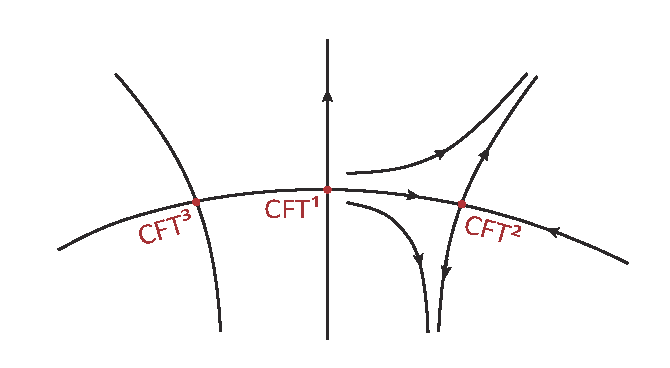
\includegraphics[width=10cm]{picture/parameter-space}
\end{figure}

By the naive dimensional analysis, the possible parameter space become finite-dimensional. Although one can consider infinitely many interaction term
$$
\cS_{int}=\int d^d x\sum g_i \mathcal{O}_i(\phi)~,
$$
the terms $\cO_i$ with $d<\Delta^i$ are suppressed at low energy, which are called \textbf{irrelevant}. Therefore, we just need to consider finitely many terms $\cO_i$ with $d\ge\Delta^i$ at low energy. To understand the behavior of a theory for these terms, we need to consider
 the beta function $\beta(g)$ describing the dependence of a coupling parameter on some energy scale $\mu$:
\begin{equation}
\beta(g)=\frac{\partial g}{\partial \log(\Lambda)}=\Lambda \frac{\partial g}{\partial \Lambda}.
\end{equation}
This implies that classical conformal invariance do not maintain conformal invariance quantum mechanically. For example, $\phi^4$ theory in $d=4$ dimensions can be shown to have the one-loop $\beta$-function
$$
\beta(\lambda)=\frac{3}{16\pi^2}\lambda^2.
$$
As we will soon see, the positive sign on this expression means the coupling constant increases with energy. These contrast with the one-loop QCD $\beta$-function,
$$
\beta(g)=-\frac{9g^3}{16\pi^2}.
$$
This $\beta$-function says the coupling decreases with energy, which is known as \textbf{asymptotic freedom}. Each of these theories, although fine classically, have length scales introduced through quantum effects. However,  if $\beta=0$,  the coupling is a constant so that the theory is scale-invariant and does not change with energy scale. The coupling constant $g^*$ with $\beta(g^*)=0$ is called \textbf{Wilson-Fischer fixed point}, and the theory at the fixed point is believed to have conformal symmetry. Therefore, conformal field theories appear at special points in the parameter spaces of quantum field theories, and they play an important role to understand families of quantum field theories. 
\begin{figure}[h]\centering
\includegraphics[width=7cm]{picture/RG}
\includegraphics[width=9cm]{picture/gapless}
\end{figure}

As we will see below, conformal field theories have more enhanced symmetries than general quantum field theories. Moreover, 2d CFTs are special because conformal symmetry becomes infinite-dimensional. In this lecture, we will study 2d CFTs by making full use of an infinite-dimensional symmetry. However, even in higher dimensions, conformal symmetries are so powerful that they provides great insights into QFTs. Moreover, if a CFT is endowed with enough supersymmetry, it is so much under control that recent study reveals some aspects of QFTs without Lagrangian description. 

\subsection{Critical phenomena}

Let us recall the basics of statistical mechanics. 
The partition function is defined by
$$
\mathcal{Z}=e^{-F/T}=\sum_{i} \exp \left(-\frac{\cE_i}{T} \right)
$$
where $F$ is called the free energy and and we set the Boltzmann constant $k_B=1$. Then, the probability $P_i$ that the system is in a state with energy $\cE_i$ is given by the Boltzmann distribution
$$
P_i=\frac1\cZ \exp(-\frac{\cE_i}{T})~.
$$
Therefore, the expectation value of an operator $\cO$ is given by
$$
\langle \cO \rangle=\frac{1}{\mathcal{Z}} \sum_{i}  \cO_i  ~ e^{- \cE_i / T} 
$$
For instance, the average energy is 
$$
E=\langle\cE\rangle=-T^2\frac{\partial}{\partial T}\left(\frac{F}{T}\right)= \frac{1}{\mathcal{Z}} \sum_{i}  \cE_i  ~ e^{- \cE_i / T} 
$$

\begin{figure}[h]\centering
\includegraphics[width=8cm]{picture/Types_of_Magnetism}
\end{figure}

Now we consider the \textbf{Ising model}  of a $d$-dimensional lattice $\Lambda$ with  $N$ lattice sites. For each lattice site $k \in \Lambda$, there is a discrete variable $\sigma_k\in  \{+1, -1\}$, representing the site's spin configuration.
The Hamiltonian of the Ising model is given by
\be\label{Ising-Hamiltonian}
\mathcal{H}=- J \sum_{\left\langle i , i^{\prime} \right\rangle} \sigma_{i} \sigma_{i^{\prime}}-B \sum_{i} \sigma_{i}
\ee
where $B$  is the external magnetic field. If $J > 0$, the alignment of spins is energetically favored and the configuration is called \textbf{ferromagnetic}. On the other hand, if $J<0$, the configuration is called \textbf{antiferromagnetic}. In the following, we will focus on the case $J>0$.


At low temperature $T$, the system settles in one of two ground states. Therefore, the magnetization $M$ has a jump discontinuity across the line of \textbf{first-order} transitions at $B=0$. A \textbf{first-order} phase transitions are the ones in which some first derivative of the free energy $F$ is discontinuous. In this example, the average energy $E$ is discontinuous. 





On the other hand, the thermal fluctuations dominate at high $T$ and spins are randomly oriented (\textbf{pramagnetic}). Therefore, there is a phase transition at the critical temperature $T=T_c$ called \textbf{Curie temperature}. The magnetization is discontinuous across the phase transition, which is called the \textbf{order parameter} of the Ising model. 


\begin{figure}[h]\centering
\includegraphics[width=5cm]{picture/1st-order-PT}
\includegraphics[width=11cm]{picture/curie}
\end{figure}

To describe this critical point, we need to introduce a notion of correlation functions.  A two-point correlation function is defined as
$$
G(r)=\left\langle \sigma_{i} \sigma_{j} \right\rangle-\left\langle \sigma_{i} \right\rangle \left\langle \sigma_{j} \right\rangle \approx r^{- \tau} \mathrm{e}^{- r / \xi}
$$
where $r=|i-j|$ is the distance between the sites $i$ and $j$. In the 2d Ising model, one has $\tau =1/2$ for $T>T_c$ and $\tau =2$ for $T<T_c$.
If $r<\xi$, the two spins are correlated, since there is a large probability that they have the same value. 
On the other hand, for sufficiently large $r\gg \xi$, probability should decrease roughly exponentially with $r$. Hence, the mean cluster size of correlated spins is  $\xi$, which is called the \textbf{correlation length}. As a temperature $T$ approaches $T_c$, the correlation length $\xi$ diverges, and such a critical point is called  \textbf{second-order}. At the critical point,  fluctuations on all length scales become important, and therefore the spin configuration is a fractal-like structure (Figure \ref{fig:fractal}). Consequently, the corresponding mass scale $1/\xi$ disappears and physics is described by conformal field theory at the critical point \cite[ISZ88-No.2]{Cardy:1984bb}.





\begin{figure}[h]\centering
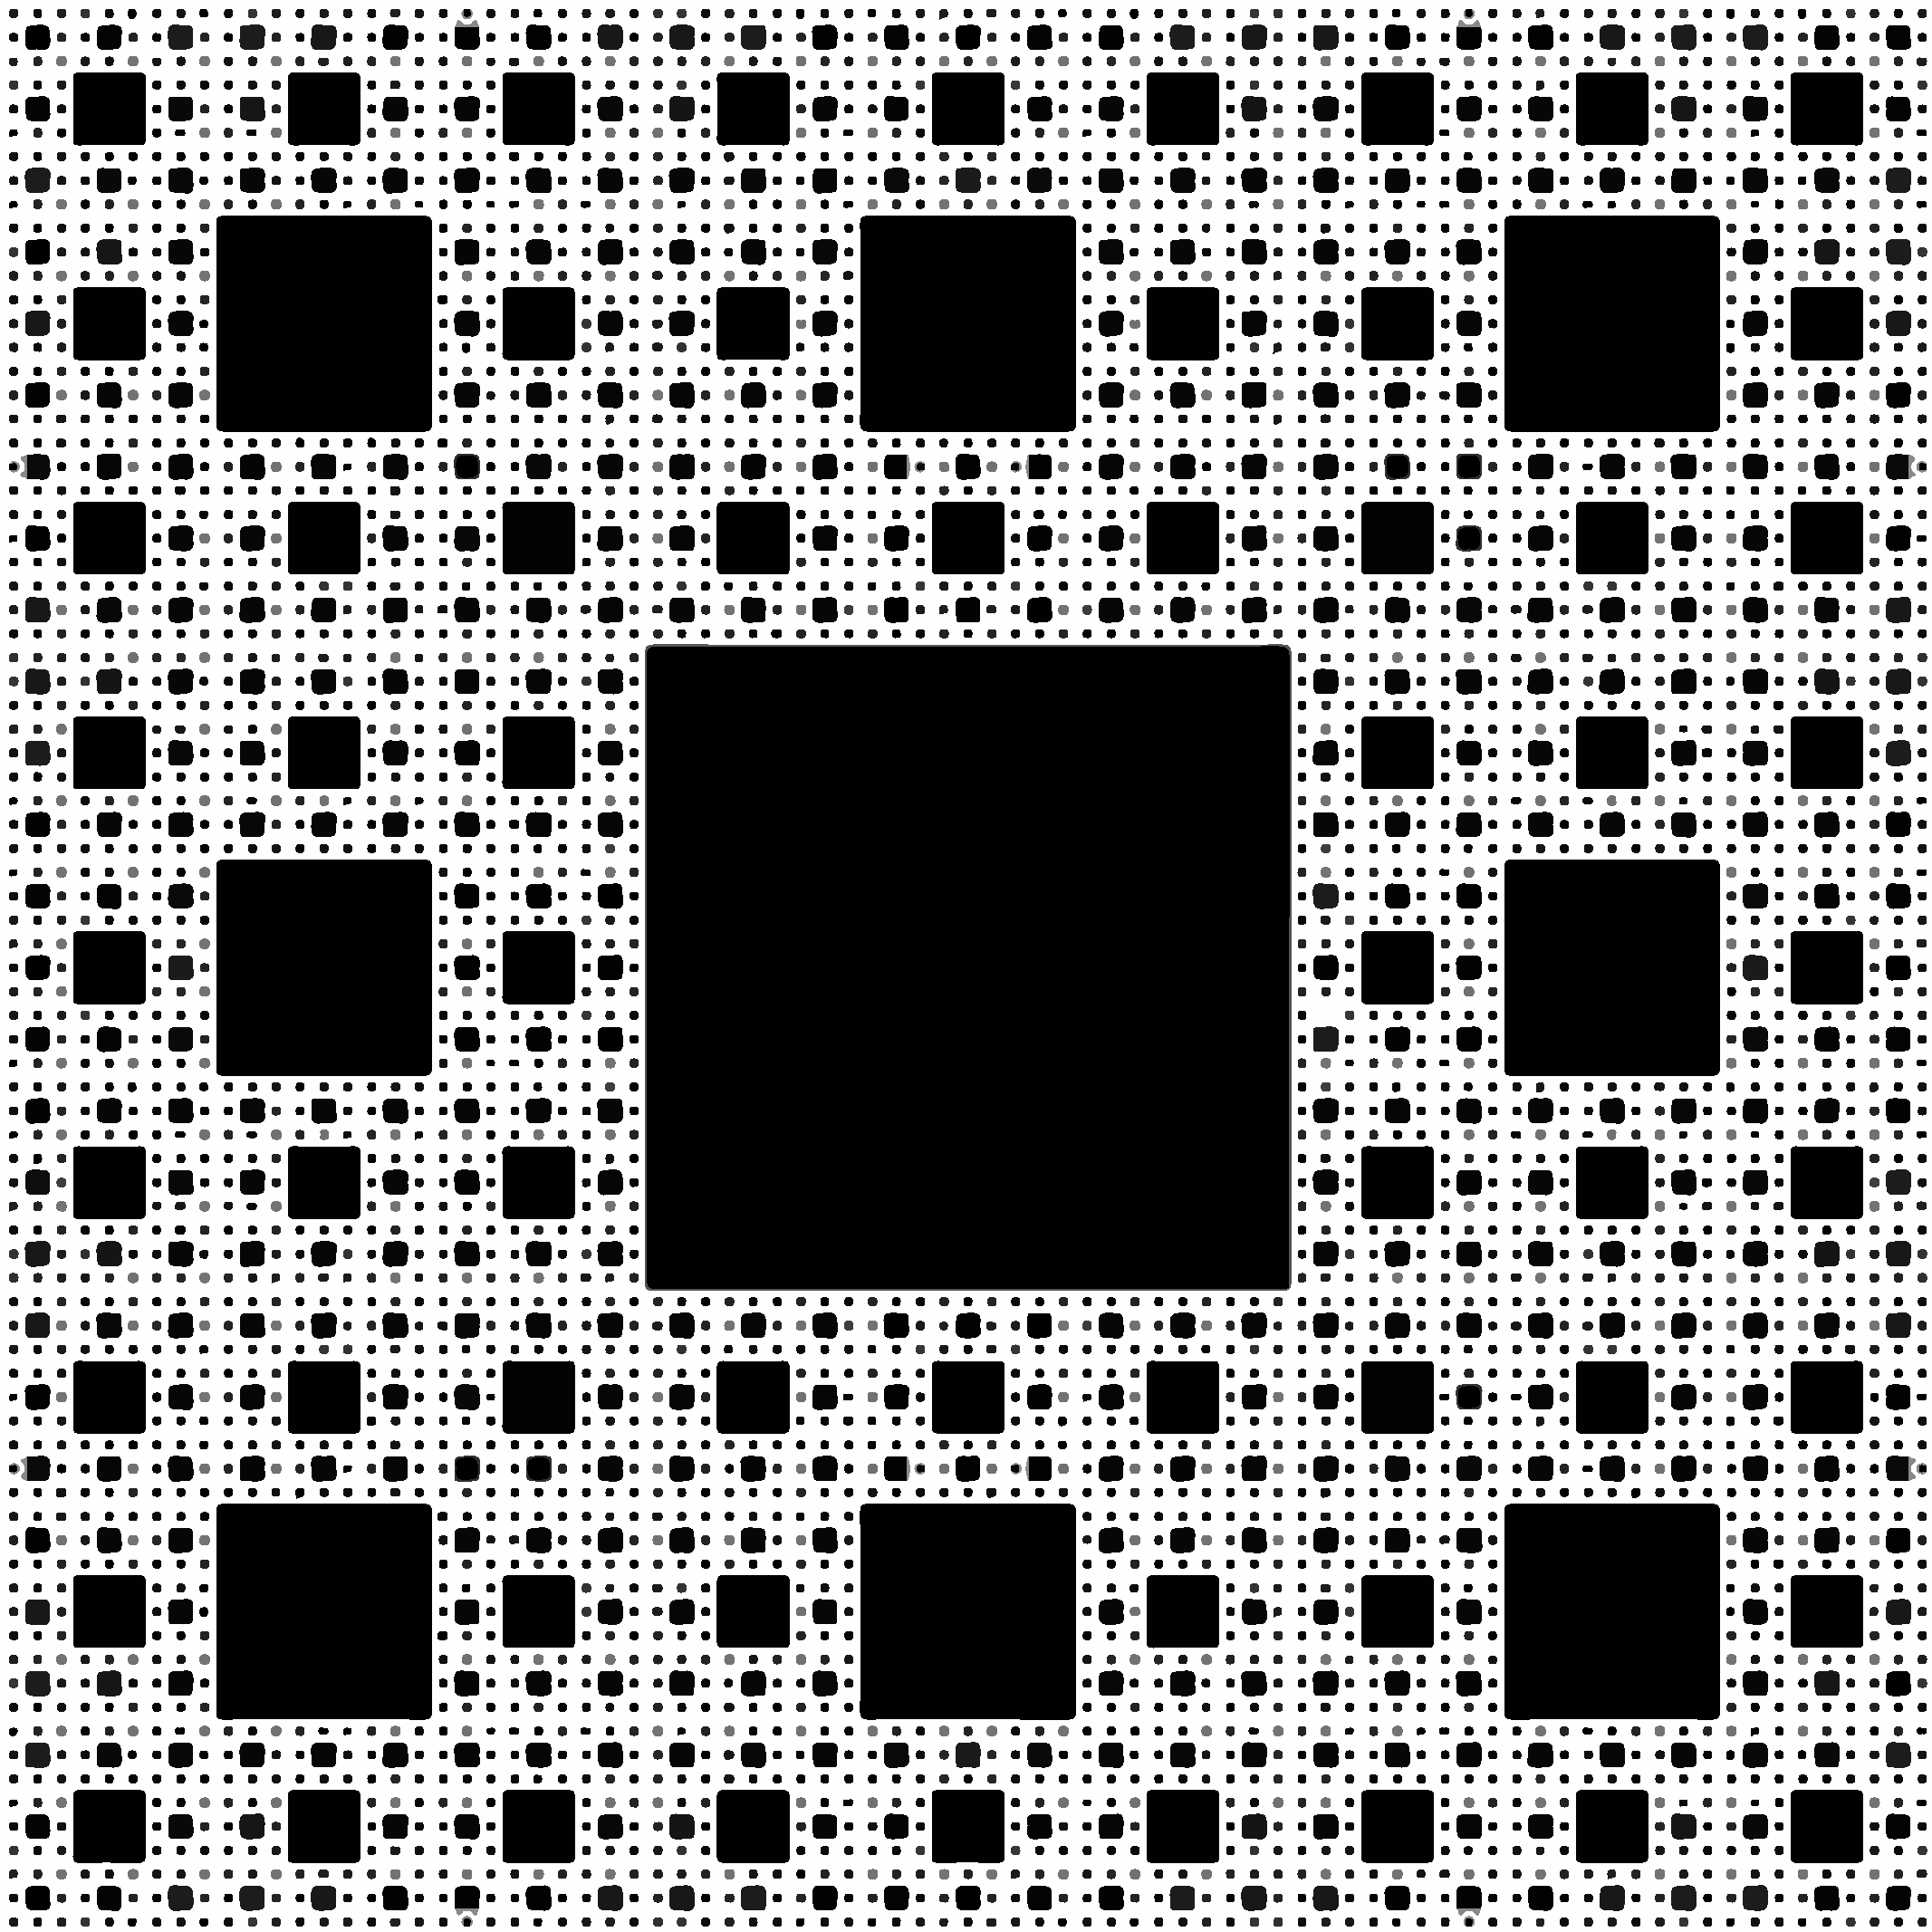
\includegraphics[width=6cm]{picture/fractal}
\caption{Schematic illustration of spin configuration at the Curie temperature $T_c$. The figure is taken from \href{https://en.wikipedia.org/wiki/Fractal}{Wikipedia:Fractal}}\label{fig:fractal}
\end{figure}


Close to the critical point, the correlation lengths and the thermodynamic quantities obey power laws, and the critical behavior near to the critical points can be  characterized by the values of the \textbf{critical exponents}. 
Introducing the reduced temperature $t$ and the reduced magnetic field $h$
$$
t :=\frac{T-T_{c}}{T_{c}} \quad \text{and} \quad h :=\frac{B}{T_{c}}~,
$$
the conventional critical exponents $\a,\b,\g,\d,\nu,\eta$ are now defined by
$$
\begin{matrix}
C \sim t^{-\alpha}&(h=0)&\textrm{specific heat}\\
M \sim (-t)^\beta &(t < 0, h=0)&\textrm{spontaneous magnetization}\\
\chi \sim t^{-\gamma}&(h=0)&\textrm{zero field susceptibility}\\
M=h^{1/\delta} &(t=0)&\textrm{magnetization}\\
\xi \sim t^{-\nu}&(h=0)&\textrm{correlation length}\\
G(r) \sim  |r|^{2-d-\eta}  &(t=0,h=0)&\textrm{2pt-function}\end{matrix}
$$
where $$
C :=-\frac{T}{N} \frac{\partial^{2} F}{\partial T^{2}} , \quad M :=-\frac{1}{N} \frac{\partial F}{\partial B} \quad , \quad \chi:=\frac{\partial M}{\partial B}~.
$$
In fact, there are relations among these critical exponents and there are only two independent exponents $\nu,\eta$. In the 2d Ising model, one has
$$
\a=0~,\quad \b=\frac18~,\quad \g=\frac74~, \quad \d=15~, \quad \nu=1~, \quad \eta=\frac14
$$
Remarkably, the critical exponents stay the same even if we change the shape of lattice or we include next-nearest-neighbor interactions. 
The independence of the critical exponents from such microscopic details is referred to as \textbf{universality}.

At the critical point, the two-point function can be written as
$$
\langle \sigma(x)\sigma(0)\rangle=\frac{C}{|x|^{2\Delta_\sigma}}
$$
where $\Delta_\sigma$ is called the \textbf{scaling dimension} of $\sigma$. 
One can similarly define a local energy density operator 
$$
\varepsilon_{i}=\sum_{i^{\prime}} J \left(i , i^{\prime} \right) \sigma_{i} \sigma_{i^{\prime}}~.
$$
Then, in the 2d Ising model, their scaling dimensions are 
\be\label{Ising-conf-dim}\Delta_\sigma =1/8~,\qquad \Delta_\e: =1~,\ee 
which we will see in the subsequent lectures.

\subsection{String theory}
Conformal field
theories play a central role in string theory \cite{GSW,Polchinski}. In string theory, string theory propagation on a certain manifold $M$ is described by a non-linear sigma model $\Sigma\to M$ where $\Sigma$ is a two-dimensional Riemann surface and $M$ is a certain manifold.  For instance, in a bosonic string theory, the action is expressed as
\bea\nonumber
 &\cS=\frac{1}{4\pi \alpha'} \int d^2x \left(\sqrt h h^{ab} \partial_a X^\mu \partial_b X^\nu G_{\mu\nu}(X)
 +i \varepsilon^{ab} \partial_a X^\mu \partial_b X^\nu B_{\mu\nu}(X)
 +\alpha' \sqrt h R^{(2)} \Phi(X)
 \right) \ .
\eea
where $h$ and $G$ are the metrics of $\Sigma$ and $M$, respectively, and  $B$ is an anti-symmetric field. To describe a consistent string theory, it must be a conformal
field theory. To preserve conformal invariance at quantum level, $M$ has to be 26-dimensional in bosonic string theory, and 10-dimensional in a string theory with supersymmetry. Moreover,  the vanishing one-loop renormalization group beta-functions of the non-linear sigma model implies that $M$ must be Ricci-flat. 


In particular, Calabi-Yau sigma models are described by $\cN=2$ superconformal field theories. It was discovered that $\cN=2$ superconformal field theories associated to a pairs of Calabi-Yau manifolds are equivalent.  
The existence of such pairs of Calabi-Yau manifolds with specified properties are known to mathematicians as the \textbf{mirror symmetry conjecture}, which is now the active subject in mathematics.

Moreover,  the equivalence between string theory on an anti-de Sitter space and conformal field theories was proposed, which is called the \textbf{AdS/CFT correspondence}. For example, this correspondence states that  non-perturbative definition of superstring theory of type IIB on AdS${}_5$ is described by the four-dimensional $\cN=4$ superconformal field theory. The AdS/CFT correspondence has been extensively studied in the last two decades, and now it has huge impact on various areas in physics. 



\subsection{References}



There are too many references on 2d CFTs and each book deals with only a certain aspect of the huge subject. 
In this lecture, we will first follow \cite{cardy1988conformal,ginsparg1988applied,zamolodchikov1989conformal}, and the yellow book \cite{francesco2012conformal} can be used as a dictionary. In addition,  we list some standard references related to
statistical mechanics \cite{cardy1996scaling,henkel2013conformal}, string theory \cite{Blumenhagen:2009zz,schellekens1996introduction,ketov1995conformal}, integrable systems \cite{gomez2005quantum,mussardo2010statistical}. In mathematics, studying the representation theoretic aspect of 2d CFTs has been led by Kac \cite{kac1994infinite}. Moreover, after the mathematical foundation of 2d CFTs has been given in \cite{segal1988definition} and \cite{tsuchiya1989conformal} (included in \cite{jimbo2014integrable}), 2d CFTs have shed drastically new insights in various aspects of modern mathematics
such as vertex operator algebras, moduli spaces, low-dimensional topology, geometric representation theory (for instance, see \cite{frenkel1989vertex,kohno2002conformal,frenkel2004vertex,beilinson2004chiral}). For  general conformal field theories of higher dimensions, we refer the reader to \cite{Nakayama:2013is,Qualls:2015qjb,Rychkov:2016iqz,Simmons-Duffin:2016gjk}

After this course, the reader would be highly recommended to read some of important original papers in \cite{itzykson1988conformal} so that the relevant papers in \cite{itzykson1988conformal} are indicated in this lecture note.  Related but more mathematical papers are collected in \cite{jimbo2012conformal,jimbo2014integrable}. Even in this fast-moving community, the importance of reading the classics cannot be overemphasized.

\section{Conformal invariance}

\subsection{Conformal Transformation}

A conformal transformation
is generally defined as follows:
Let us consider differentiable map 
$\phi : U \rightarrow V$, 
where $U$ and $V$
are  open subsets of 
$M$ and $M'$ respectively.
Denoting $g$ and $g'$ as the metric tensors of 
$M$ and $M'$ respectively,
we can pull back $g'$ by using the map $\phi$, 
as we have learnt in differential geometry. 
A conformal transformation 
is then defined by such a map 
that its pull back metric 
$\phi^{*} g'$ 
satisfying the following condition:
\begin{equation}
  \phi^{*}g'=\Lambda g \, .
\end{equation}
Denoting 
$x'=\phi(x)$ 
with $x \in U$, 
we can express the condition in a covariant form:
\begin{equation}
\label{general-def-ct}
g'_{\rho\sigma}(x')
\pdv{x'^{\rho}}{x^\mu}
\pdv{x'^\sigma}{x^\nu}
=
\Lambda(x)g_{\mu\nu}(x)
\,,
\end{equation}
where $\Lambda(x)$ is a positive scalar
called the scale factor. 
We see an appreciable extrapolation 
from \eqref{general-def-ct}, 
that any smooth transformation in one dimension
is a conformal transformation.
In addition, by using 
\eqref{general-def-ct}, 
the inner product of two arbitrary vectors $V'^{\mu}_{1}(x')$ 
and $V'^{\mu}_{2}(x')$ 
at the same point of $M'$
has a scaling effect 
after its pulling back
by the conformal map:
\begin{equation}
  \label{inner-product-relation}
  g_{\mu\nu}(x)V_1^\mu(x)V_2^\nu(x)
  =
  g'_{\mu\nu}(x')V'^\mu_1(x')V'^\nu_2(x')
  \Lambda
  \, ,
\end{equation} 
where $V^{\mu}_{1}(x)$ 
and $V^{\mu}_{2}(x)$ 
are the pull-back vectors respectively.
From \eqref{inner-product-relation},
it is not difficult to find that 
the included angle
of two vectors 
of $M'$ remains the same 
when they are pulled back 
by a conformal map to $M$.

In this lecture note, we focus on 
$M'=M$, which implies g'=g. 
We also consider $M$ to be flat spaces 
with a constant metric 
$\eta_{\mu\nu} 
= 
\text{diag}(-1,\dots,+1,\dots)$.
Thus, the condition for  
a conformal transformation 
can be written as 
\begin{equation}
\label{def-flat-ct}
\eta_{\rho\sigma} 
\pdv{x'^\rho}{x^\mu}
\pdv{x'^\sigma}{x^\nu}
=
\Lambda(x)\eta_{\mu\nu}
\, .
\end{equation}
The line element transforms 
under conformal transformation as
\begin{equation}
  \dd s^2 
  =
  \eta_{\mu\nu}
  \dd x^\mu \dd x^\nu
  \rightarrow 
  \eta_{\rho\sigma}
  \dd x'^\rho \dd x'^\sigma
  =
  \eta_{\rho\sigma}
  \pdv{x'^\rho}{x^\mu}
  \pdv{x'^\sigma}{x^\nu}
  \dd x^\mu \dd x^\nu
  =\Lambda(x)\dd s^2
  \, .
\end{equation} 
Two remarks should be stated here. 
First of all, 
using \eqref{def-flat-ct},
we can see 
the composition of 
two conformal transformation 
is still conformal, 
which may imply that
conformal transformations form 
a group.
Secondly, 
the scale factor  
$\Lambda(x)=1$
corresponds to the Poincare group.
   
\subsection{Conditions for Conformal Invariance}
In this part, we need to figure out
some basic conformal transformations 
in flat space. To begin with, 
we study the infinitesimal transformations
\begin{equation}
 x'^\rho=x^\rho+\e^\rho(x)+O(\e^2)
 \, ,
\end{equation} 
with an infinitesimal variable 
$\e(x)\ll1$. 
Plugging into the conformal condition
\eqref{def-flat-ct}, 
up to first order in $\e$, 
the infinitesimal form 
of conformal transformation 
may be derived as:
\begin{equation}
\label{inf-constraint-K}
  \partial_{\mu}\e_\nu
  +
  \partial_{\nu}\e_\mu
  =
  K(x) \eta_{\mu\nu} 
  \, ,
\end{equation} 
with $K(x)=\Lambda(x)-1$, 
some infinitesimal function. 
However, since we want to find out 
the explicit form for 
$\e(x)$,
$K(x)$ need to be cancelled 
in the constraint formula.
By tracing both sides of
\eqref{inf-constraint-K},
we have
\begin{equation} 
  K(x)
  =
  \frac{2 \partial^{\mu}\e_\mu}
 {d} 
  \, .
\end{equation}
Plugging back to
\eqref{inf-constraint-K}, 
we find the restriction depending on 
$\e(x)$ 
to make the transformation conformal:
\begin{equation}
\label{inf-cft-e-condition}
  \partial_{\mu}\e_\nu
  +
  \partial_{\nu}\e_\mu
  =
  \frac{2}{d}
  (\partial\cdot\e)
  \eta_{\mu\nu}
  \, .
\end{equation}

\subsection{Some Useful Relation}

Let us derive two useful equations 
for later purpose.
First of all, by taking 
$\partial^{\nu}$
to both sides of 
\eqref{inf-cft-e-condition},
we can obtain
\begin{equation}
  \partial_{\mu}
  (\partial\cdot\e)
  +
  \square\e_\mu
  =
  \frac{2}{d}
  \partial_{\mu}
  (\partial\cdot\e)
  \, .
\end{equation}
We then take $\partial_{\nu}$
to both sides:
\begin{equation}
\label{inf-cft-e-condition-2}
  \partial_{\mu}\partial_{\nu}
  (\partial\cdot\e)
  +
  \square
  \partial_{\nu}\e_\mu
  =
  \frac{2}{d}
  \partial_\nu\partial_{\mu}
  (\partial\cdot\e)
  \, .
\end{equation}
Interchanging 
$\mu \leftrightarrow \nu$,
adding back to
\eqref{inf-cft-e-condition-2}
and using 
\eqref{inf-cft-e-condition} 
we get
\begin{equation}
  \label{e-useful-relation-1}
  (
   \eta_{\mu\nu}\square
   +
   (d-2)
   \partial_{\mu}\partial_{\nu}
 )
  (\partial\cdot\e)
  =
  0
  \, .
\end{equation}
Finally, tracing spacetime indices gives
\begin{equation}
  \label{e-useful-relation-2}
  (d-1)\square
  (\partial\cdot\e)
  =
  0
  \, .
\end{equation}

The second useful expression 
is obtain by taking 
$\partial_{\rho}$ of
\eqref{inf-cft-e-condition}
and permuting indices:
\bea
  \partial_{\rho}
  \partial_{\mu}
  \e_\nu
  +
  \partial_{\rho}
  \partial_{\nu}
  \e_\mu
  &=
  \frac{2}{d}
  \eta_{\mu\nu}
  \partial_{\rho}
  (\partial\cdot\e)
  \, ,
  \notag 
  \\
  \partial_{\nu}
  \partial_{\rho}
  \e_\mu
  +
  \partial_{\mu}
  \partial_{\rho}
  \e_\nu
  &=
  \frac{2}{d}
  \eta_{\rho\mu}
  \partial_{\nu}
  (\partial\cdot\e)
  \, ,
  \notag 
  \\
  \partial_{\mu}
  \partial_{\nu}
  \e_\rho
  +
  \partial_{\nu}
  \partial_{\mu}
  \e_\rho
  &=
  \frac{2}{d}
  \eta_{\nu\rho}
  \partial_{\mu}
  (\partial\cdot\e)
  \, .
  \notag 
\eea
Subtracting the first line from
the sum of the last two leads to
\begin{equation}
\label{inf-cft-e-relation-3}
  2\partial_{\mu}
  \partial_{\nu}
  \e_\rho
  =
  \frac{2}{d}
  (
   -
   \eta_{\mu\nu}
   \partial_\rho
   +
   \eta_{\rho\mu}
   \partial_{\nu}
   +
   \eta_{\nu\rho}
   \partial_{\mu}
 )
  (\partial\cdot\e)
  \,
  .
\end{equation}

\subsection{Conformal Transformation in $d \geq 3$}\label{sec:conf-gen}

For the case $d=1$, 
the relation
\eqref{e-useful-relation-2}
imposes no constraint to 
$\e(x)$,
which accords with 
what we have claimed, 
that any smooth  
transformation in one dimension 
is conformal.
The case $d=2$
will be studied later
in detail.
In this section, 
let's focus on the case 
$d\geq 3 $.

According to 
\eqref{e-useful-relation-2} for 
$d \geq 3$, we have 
$\square (\partial\cdot\e)=0$. 
Substituting back to condition
\eqref{e-useful-relation-1}
gives 
$
 \partial_{\mu}
 \partial_{\nu}
 (\partial\cdot\e)
 =
 0
$
,implying that
$(\partial\cdot\e)$
is at most linear in
$x^\mu$,
i.e. 
$
 (\partial\cdot\e)
 =
 A+B_{\mu}x^\mu
$
.When plugging this linear expression 
back to 
\eqref{inf-cft-e-relation-3},
we immediately obtain that 
$
 \partial_{\mu}
 \partial_{\nu}
 \e_\rho
$
equals to a constant.
This follows that 
$\e_\mu$
is at most quadratic in
$ x^{\nu}$
and so we can make the ansatz:
\begin{equation}
\label{e-ansatz}
  \e_\mu
  =
  a_\mu
  +
  b_{\mu\nu} x^\nu
  +
  c_{\mu\nu\rho}x^\nu x^\rho
  \, ,
\end{equation}
where, 
$ c_{\mu\nu\rho}
=
c_{\mu\rho\nu}
$.
For the infinitesimal nature of 
$\e_\mu$, 
all the constants:
$ 
 a_\mu,b_{\mu\nu},c_{\mu\rho\nu}
 \ll 1
$.

Noticing that all the terms in
\eqref{inf-cft-e-condition},
have only one derivative, 
and that the conformal constraints
for these constants should be 
independent of 
$x^\mu$, 
we can study the various terms in
\eqref{e-ansatz} separately.

The constant term $a_\mu$ in
\eqref{e-ansatz} 
is not constrained by
\eqref{inf-cft-e-condition}.
It describes infinitesimal translation
$x'^\mu=x^\mu+a^\mu$,
for which the generator is
the momentum operator 
$P_\mu=-i\partial_{\mu}$
\footnote{
	All the generators of this form can be calculated by the definition :
	\begin{equation}
	  \label{def-generator}
	  iG_a\Phi
	  =
	  \frac
	 {\delta x^\mu}
	 {\delta \omega_a}
	  \partial_{\mu}
	  \Phi
	  \, ,
	\end{equation}
	if we suppose that the fields are not affected by the transformation with $\omega_a$ the corresponding parameter. 
}.

Inserting the linear term into 
\eqref{inf-cft-e-condition}
, we find
\begin{equation}
\label{linear-condition}
  b_{\mu\nu}
  +
  b_{\nu\mu}
  =
  \frac{2}{d}
  (
   \eta^{\rho\sigma}
   b_{\sigma\rho}
 )
  \eta_{\mu\nu}
  \, .
\end{equation}
We then split $b_{\mu\nu}$ into
symmetric and antisymmetric part, i.e.
$b_{\mu\nu}=n_{\mu\nu}+m_{\mu\nu}$, 
with
$n_{\mu\nu}=n_{\nu\mu}$ 
and
$m_{\mu\nu}=-m_{\nu\nu}$.
The antisymmetric part 
$m_{\mu\nu}$
satisfy 
\eqref{linear-condition} 
automatically, while 
the symmetric part gives constraint:
$
 n_{\mu\nu}
 =
 \frac{1}{d}
 (
  \eta^{\rho\sigma}
  n_{\sigma\rho}
)
 \eta_{\mu\nu}
$
, telling that the symmetric part
should be diagonal.
Therefore, we can split  
$b_{\mu\nu}$ as
\begin{equation}
	b_{\mu\nu}
	=
	\alpha\eta_{\mu\nu}
	+
	m_{\mu\nu}
	\, .
\end{equation}
The symmetric term 
$\alpha\eta_{\mu\nu}$
describes infinitesimal 
scale transformation
$
 x'^\mu
 =
 (1+\alpha)x^\mu
$
with generator
$
  D= -ix^\mu\partial_\mu
$.
The antisymmetric part 
$m_{\mu\nu} $
corresponds to infinitesimal
rotations
$
  x'^\mu
  =
  (
   \delta^\mu_\nu
   +
  {m^\mu}_\nu
 )
  x^\nu
$
with generator being the
angular momentum operator 
$
  L_{\mu\nu}
  =
  i(
  x_\mu\partial_\nu
  -
  x_\nu\partial_\mu
 )
$.


Now let us consider the quadratic term.
By inserting the quadratic term into
\eqref{inf-cft-e-relation-3}, after straight-forward calculation, 
we find that
\begin{equation}
  c_{\mu\nu\rho}
  =
  \eta_{\rho\mu}f_\nu
  +
  \eta_{\mu\nu}f_\rho
  -
  \eta_{\nu\rho}f_\mu
  \, ,
\end{equation}
with 
$f_\mu=\frac{1}{d}{c^\rho}_{\rho\mu}$.
The resulting transformations are
\begin{equation}
\label{inf-SCT}
  x'^\mu 
 =
  x^\mu
  +
  2(x\cdot f)x^\mu
  -(x\cdot x)f^\mu
  \, ,
\end{equation}
which are called 
\textbf{special conformal transformations}
(SCT)
and the corresponding generator is 
$
 K_\mu
=
 -i(
     2 x_\mu x^\nu\partial_\nu
     -
     (x\cdot x)\partial_{\mu}
)
$
.

\subsection{Finite Conformal Transformation}
So far, we have identified 
all basic infinitesimal conformal transformations 
and their generators. 
However, in order to determine 
the conformal group,
we also need the corresponding
finite transformations. 
All the basic
finite conformal transformations
are shown in Table \ref{Tab:fin-ct}.
\begin{table}[htbp]
	\centering
	 \caption{Finite conformal transformations
	 and corresponding generators}
	 \label{tab:ModelASymbol}
	 \begin{tabular}{lll}
	 	\toprule
	 	  Transformations 
	 	&
	 	& Generators 
	 	\\
	 	\midrule
	 	  translation
	 	& $x'^\mu=x^\mu+a^\mu$
	 	& $P_\mu=-i \partial_\mu$ 
	 	\\
	 	  dilation
	 	& $x'^\mu= \alpha x^\mu$
	 	& $D=-ix^\mu
	 	   \partial_\mu
	 	  $
	 	\\
	 	  rotation
	 	& $x'^\mu 
	 	   ={M^\mu}_\nu x^\nu
	 	  $
	 	& $L_{\mu\nu}=
	 	   i(
	 	   x_\mu\partial_\nu
	 	   -
	 	   x_\nu\partial_\mu
	 	  )
	 	  $
	 	\\
	 	  SCT
	 	& $x'^{\mu}=
	 	   \frac
	 	  {x^\mu-(x\cdot x)f^\mu}
	 	  {
	 	   	1-2(f\cdot x)
	 	   	+
	 	   	(f\cdot f)(x\cdot x)}
	 	  $
	 	& $K_\mu=-i(
	 	   2 x_\mu x^\nu\partial_{\nu}
	 	   -
	 	   (x\cdot x)\partial_\mu
	 	  )
	 	  $
	 	\\
	 	\bottomrule                
	 \end{tabular}\label{Tab:fin-ct}
\end{table} 
The finite transformations 
for translation and rotation 
are Poincare transformations
we are familiar with.
The finite transformation for 
dilation can be derived from
it infinitesimal  form easily.
Thus, what we focus on is 
the finite transformation 
for SCT.
It is hopeless to derive it 
through its infinitesimal form.
But, we can guess this finite 
form of transformation, 
if we realize that an inversion 
$x'^\mu=\frac{x^\mu}{x\cdot x}$
is also a conformal map. By plugging
in to \eqref{def-flat-ct}, 
we can obtain its scale factor as
$\Lambda(x)=(x\cdot x)^{-2}$. 
Inversion can be one of the
basic finite conformal transformation
instead of SCT. 
However, it has neither 
infinitesimal form nor parameters. 
Now we want to
construct finite SCT. 
Using the transitive property
for conformal map,
we can thus first make 
an inversion of  
$x^\mu$, then
make an translation 
$f^\mu$,
and inverse the result again
to construct a new 
conformal transformation. 
An illustration in two dimensions
is shown in
Figure \ref*{fig:SCT-ill}.
As $f^\mu$ goes to zero, 
$x^\mu$ maps to itself. 
Therefore it should have 
infinitesimal form. 
\begin{figure}[h]
	\centering  
	\includegraphics
	[width=0.7\linewidth]
	{picture/SCT-ill.pdf} 
	\caption
	{
		Illustration of a finite
		Special Conformal 
		Transformation 
	}  
	\label{fig:SCT-ill}   
\end{figure}
\begin{equation}
\label{fin-SCT}
  x'^\mu 
 =\frac
   {
      \frac{x^\mu}{x\cdot x}
      -f^\mu
  }
   {
      (\frac{x^\mu}{x\cdot x}
      -f^\mu)
      (\frac{x^\mu}{x\cdot x}
      -f^\mu)
  }
 =\frac
   {x^\mu-(x\cdot x)f^\mu}
   {
  	 1-2(f\cdot x)
  	 +
  	 (f\cdot f)(x\cdot x)
  }
    \, .
\end{equation}
The result is what we have shown in 
Table \ref{Tab:fin-ct}. 
It is easy to verify that
when $f^\mu \rightarrow 0$,
\eqref{fin-SCT} reduces to
infinitesimal form of SCT: 
\eqref{inf-SCT}.   
Further more
by using 
\eqref{def-flat-ct},
after a heavy and tedious calculation,
the scale factor for SCT 
can be computed as
\begin{equation}
  \Lambda(x)
  =
  (1-2(f\cdot x)+ (f\cdot f)(x\cdot x))^{-2}
\end{equation}
Finally, we observe from 
\eqref{fin-SCT}, 
that 
the finite SCT are not globally defined.
In particular,
for a given non-zero vector
$f^\mu$, 
there is a point 
$x^\mu=\frac{1}{f\cdot f}f^\mu$ 
such that 
$x^\mu$ 
is mapped to infinity.
(The denominator goes to 
 zero more quickly
 than the numerator.)
Therefore, in order to define
the arbitrary conformal transformation, the point at infinity should
be included. 

\subsection{Conformal Groups and Algebras}

The conformal transformations form a group, called the conformal group of dimension $d\ge3$. 
Actually,
the algebra generated by
infinitesimal conformal transformations
is the Lie algebra of the conformal group, called the
conformal algebra.

Let us identify the conformal algebra  of dimension $d\ge3$.  
The dimension of the algebra is
$N=d+1
  +\frac{d(d-1)}{2}
  +d
  =\frac{(d+2)(d+1)}{2}
$ 
by counting the generators in
Table \ref{Tab:fin-ct}.
The commutation rules
with no central charge 
can be obtained 
by direct calculations.
\bea
\label{com-rela-conf}
   \comm{D}{P_\mu}
   &=
   i P_\mu
   \notag\, ,\\
   \comm{D}{K_\mu}
   &=
   -i K_\mu
   \notag\, ,\\
   \comm{K_\mu}{P_\nu}
   &=
   2i(
   \eta_{\mu\nu}D
   -
   L_{\mu\nu}
  )
   \notag\, ,\\
   \comm{K_\rho}{L_{\mu\nu}}
   &=
   i(
   \eta_{\rho\mu}K_\nu
   -
   \eta_{\rho\nu}K_\mu
  )
   \, ,\\
   \comm{P_\rho}{L_{\mu\nu}}
   &=
   i(
   \eta_{\rho\mu}P_\nu
   -
   \eta_{\rho\nu}P_\mu
  )
   \notag\, ,\\
   \comm{L_{\mu\nu}}{L_{\rho\sigma}}
   &=
   i(
   \eta_{\rho\nu}L_{\mu\sigma}
   +
   \eta_{\mu\sigma}L_{\nu\rho}
   -
   \eta_{\rho\mu}L_{\nu\sigma}
   -
   \eta_{\nu\sigma}L_{\mu\rho}
  )
   \notag\, .
\eea
To put the above commutation relations
into a simpler form,
we define the following generators.
\bea
   &J_{\ \mu,\nu}
   =
   L_{\mu,\nu}
   \, ,\notag \\
   &J_{-1,0}
   =
   D
   \, ,\notag \\
   &J_{-1,\mu}
   =
   \frac{1}{2}
   (P_\mu-K_\mu)
   \, ,\\
   &J_{\ 0,\mu}
   =
   \frac{1}{2}
   (P_\mu+K_\mu)
   \, .\notag
\eea
By using 
\eqref{com-rela-conf},
we can verify that 
$J_{m,n}$ with
$m,n=-1,0,1,\dots d$,
satisfy the following commutation relations:
\begin{equation}
\label{simper-conf-algebra}
  \comm{J_{mn}}{J_{rs}}
  =
  i(
  \eta_{ms}J_{nr}
  +
  \eta_{nr}J_{ms}
  -
  \eta_{ms}J_{ns}
  -
  \eta_{ns}J_{mr}
 )
  \, .
\end{equation}
For Euclidean $d$-dimensional 
space $\mathbb{R}^{d}$, we see 
the metric
$\eta_{mn}$ here
is 
$\eta_{mn} =$ 
$\text{diag}(-1,1,\dots,1)$ so that
we identify 
\eqref{simper-conf-algebra}
with the commutation relations
of the Lie algebra 
$\mathfrak{so}(1,d+1)$.
We can generalize the result 
to the space $\mathbb{R}^{p,q}$,
with 
$d=p+q \geq 3$.
The corresponding conformal group
is 
$SO(p+1,q+1)$. 


\bibliography{conformal-ref}
\bibliographystyle{halpha}






\end{document}
